\chapter{History}
\subitem{
	It is known that the evolution of the Internet has been in stages. \\ Since World War II until the early nineties of the twentieth century was the uses of network for just military applications, specifically the US Army. \\ Then there was the strategic decision to open the door to use civilian applications in the late eighties and nineties of the twentieth first century. \\ And recognize a lot of the military they did not expect enormous Spread of the Internet and its services in the world, also did not expect that affects the use of all walks of life applications. \\ With the spread of cellular technology or mobile new form of technology, to exceed force of 100 per cent in many countries of the world, and the emergence of mobile technology tablet PCs and smart handheld and generations of data transfer over the phone services such as 2G, 3G, 4G, open the floodgates the expansion of the phenomenon of social networking-mail (in both audio and visual), all of that has led to the emergence of the third generation of the Internet, a generation Semantic web (semantic web). \\ This refers to the availability of Internet tools, such as search engines, means building links between the concepts and the significance of vocabulary, to convert unstructured data into structured or semi-structured data easier to use and manipulate. \\
	\\ \\ \\ \\ \\ \\ \\
	In parallel, the expansion in the use of smart equipment and supplied technologies Palmstharat algorithms and programming simple and effective devices that operate global positioning system event (GPS) and sensor technology for near and remote and connect wired and wireless, and this is what sparked great enthusiasm among individuals and institutions to take advantage of these services. \\ Which enabled the emergence of the phenomenon of communication and online communication between devices each other, and this is required.
}

\subitem{
	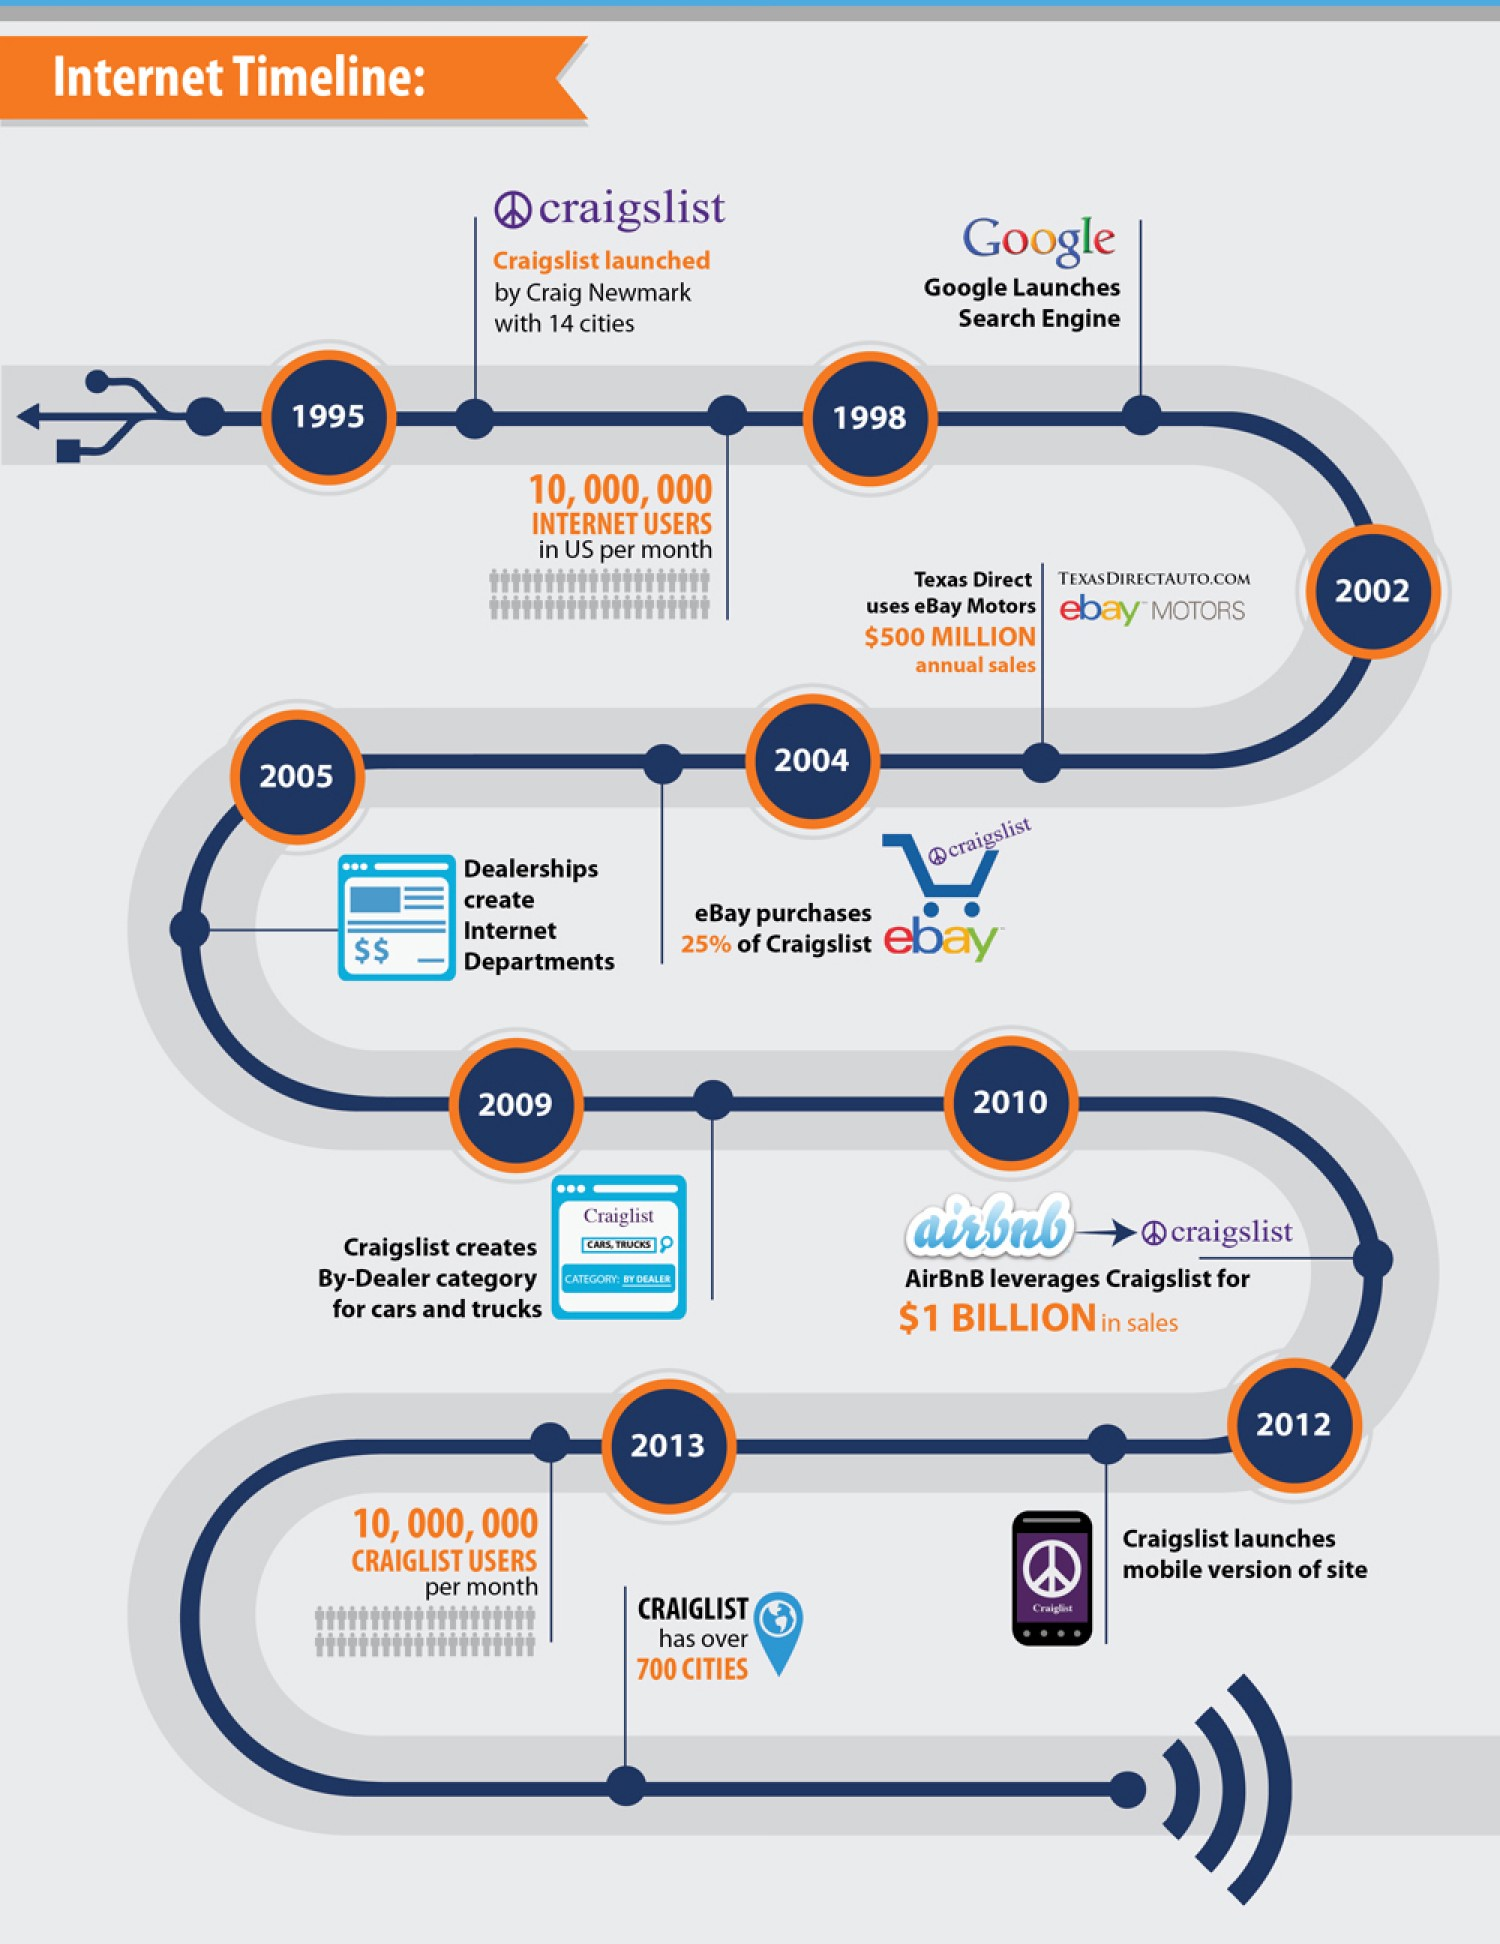
\includegraphics[width=\textwidth,height=\textheight,keepaspectratio]{IOT4.jpg}}